\chapter{Architecture \& Development}
This chapter will go into detail of the development stages of this project, discussing the various decisions, challenges and problems faced during the development of each individual component in the system, and how they were resolved.

\section{System Architecture}
% Overview of sys arch, diagram to rep the key elements

The majority of the system attempts to follow the MVC (Model-View-Controller) software architectural pattern where possible. This pattern simplifies the development of complex systems by separating the data, display and logic sections into more managable subsystems - the model, view and controller respectively. The structure and architectural pattern of each individual component in this system will be described in depth in Section \ref{section:systemcomponents}.

% ref MVC, simplifies



% Maybe show visualops.io network diagram here
% Architectural patterns used
	\subsection{Development Environment}
	% OS - Local system, Python, Pip, Virtualbox, libraries needed
	% Downloading the JS libs (Bootstrap, Handlebars, Three, Ammo, Ace, etc)
	% Sublime, GitHub, EB CLI
	% Originally one repo, split into two to make deployment easier \ref deployment


\section{System Components}
\label{section:systemcomponents}
% Details of each component, problems encountered and resolved, challenges overcome or worked around
% 
	\subsection{Storage Server}
	% - Pattern - MVC-like
	% - Why this was it's own server
	% - restful API, flask app
		% - GitPython usage
		% - git operations, access_token, remotes
	% - Talk about each API route individually

	% - mongodb
	\subsection{Web Server}
	The Flask application created for the web server uses a software architectural pattern \emph{similar} to the MVC pattern. Flask lends itself well to the MVC pattern; as each page has it's own route (\textbf{Controller}) and template (\textbf{View}), and the template can be populated with \textbf{Data} by the route. This can be seen visualised in Figure \ref{fig:flaskprocess} which demonstrates how a request is handled by Flask. A client sends a request to the route, the route then retrieves any requested data (Such as a list of published games), then it renders the template for that route with the data. The rendered HTML from the template is sent back as the HTTP response.

	\begin{figure}[h]
		\centering
		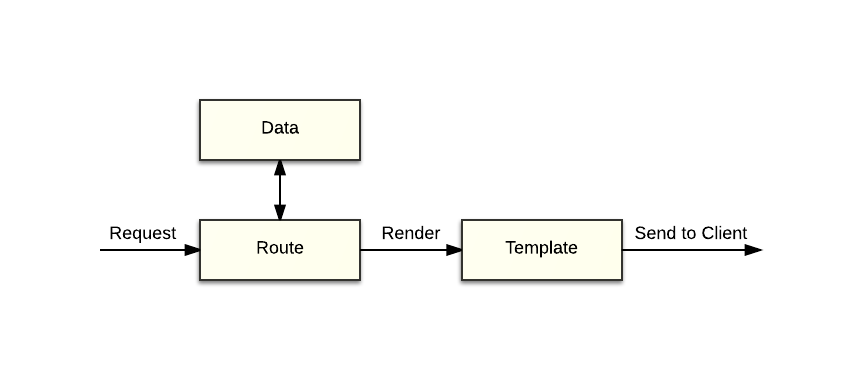
\includegraphics[scale=0.8]{flaskprocess}
		\caption{Flask request process}
		\label{fig:flaskprocess}
	\end{figure}
	% - Communication with storage server{storing remote access_token etc}
	% - GitHub API, login access_token, emails, list of repos for cloning etc
	% - Connecting to MongoDB on storage server
	\subsection{Game Engine}
	% - ECS pattern
	% - Using Three.js - structuring shit to load automatically 	into the scene etc
	% - Using Ammo.js
	% - Simplifying the two libraries into the ECS architecture
	% 	This was achieved by etc.
	% - "Game".
	% - Each pre-defined component
	\subsection{Game Editor}
	% - Pseudo MVC microframework
		% Looked at frameworks, all too heavy
		% Just made my own to keep it simple, based on something similar to backbone
	% - Detail each view
	% - Tying in the game engine with the storage backend
	% - Properties of both the gamedata json and the displayed game entities
	% - Scripts, Ace editor
	% - autosaving
	\subsection{Scalable Cloud Deployment}
	% - Setting up AWS
	% - Load balancing, separating web from storage
	% - SSH, Git, tools
	% - Deploying to Elastic Beanstalk {eb cli}
	% - Storage server {MongoDB, git, cloning the storage repo}
		% - Deployment was difficult compared to Elastic Beanstalk (used git to deploy latest version)

\section{Deployment to AWS}
% How everything was deployed etc

\section{Key Development Components}
% Identify key development components
% Key components were the game engine, editor, web server (load balancing) and storage.
% Git integration wasn't as important to functionality

\section{External APIs}
% Indentification/explanation of external APIs used vs own code. 

\section{List of Classes}
% List of classes of your code
% Write block comments for code during this process?